\chapter{Modelli} \label{ch:modelli}
In questo capitolo verranno presentati i modelli che si è deciso di addestrare
per svolgere il compito di classificazione. I modelli sono stati scelti in base
ai risultati ottenuti nella fase di analisi esplorativa e in base alle
caratteristiche del dataset. In particolare, si è deciso di addestrare:
\begin{itemize}
    \item \textbf{Support Vector Machine}
    \item \textbf{Gaussian Naive Bayes}
    \item \textbf{Rete Neurale}
\end{itemize}
Per ognuno di essi verrà presentata una breve descrizione sulla loro struttura
e sulle operazioni che sono state svolte per la loro definizione. In un secondo
momento verranno presentati i risultati ottenuti e verrà fatta una valutazione
sui modelli addestrati.

Più precisamente per ogni modello sono state addestrate due versioni, la prima
viene allenata sul dataset ridotto analizzando le correlazione, la seconda
su quello ridotto con PCA. Nella tabella \ref{tab:riassunto_operazioni_dataset} è
presente un breve riepilogo delle versioni dei dataset e dei modelli.
\begin{table}[!ht]
    \resizebox{\textwidth}{!}{\begin{tabular}{@{}llc@{}}
            \toprule
            \rowcolor[HTML]{EFEFEF}
            \textbf{Nome del dataset}                                                                                          &
            \textbf{Operazioni applicate}                                                                                      &
            \multicolumn{1}{l}{\cellcolor[HTML]{EFEFEF}\textbf{Utilizzato per i seguenti modelli}}                                                                                                      \\ \midrule
            \texttt{dataset\_corr}                                                                                             &
            \begin{tabular}[c]{@{}l@{}}Riduzione della dimensionalità utilizzando l'analisi \\ della correlazione\end{tabular} &
            GNB\_corr                                                                                                                                                                                   \\
            \texttt{dateset\_corr\_std}                                                                                        & dataset\_corr con la standardizzazione dei dati & SVM\_corr e NN\_corr \\
            \texttt{dateset\_pca}                                                                                              & dataset\_corr\_std applicando l'algoritmo PCA   & GNB\_pca             \\
            \texttt{dateset\_pca\_std}                                                                                         & dataset\_pca con la standardizzazione dei dati  & SVM\_pca e NN\_pca   \\ \bottomrule
        \end{tabular}}
    \caption{Riassunto delle operazioni effettuate sui dataset e utilizzo dei dataset per i modelli.}
    \label{tab:riassunto_operazioni_dataset}
\end{table}

Successivamente, per ogni versione di ciascun modello saranno presentate due
tipologie di valutazione delle performance:
\begin{itemize}
    \item \textbf{Valutazione $80/20$}: si effettuano gli apprendimenti di
          ciascuna versione sull'$80\%$ del dataset di riferimento e si valida
          la versione del modello sul $20\%$ del dataset di riferimento rimanente.
    \item \textbf{Cross-validation}: si effettua una $10$-fold stratified
          cross-validation per studiare la robustezza della versione del modello
          validata precedentemente.
\end{itemize}
La scelta di effettuare una valutazione in due fasi si basa sul fatto che il
numero degli esempi presenti nel dataset non è molto elevato, più precisamente
il dataset è di medie dimensioni, quindi la valutazione $80/20$ potrebbe non
essere affidabile. La seconda valutazione si effettua per verificare la
robustezza dei modelli creati, calcolando gli intervalli di confidenza delle
metriche di valutazione.

La porzione di dati dedicata all'addestramento dei modelli, composta dall'$80\%$
delle istanze, è anche stata utilizzata anche per ricercare gli iperparamentri 
migliori per la rete neurale e per la SVM, più precisamente è stato effettuati 
una $5$-fold stratified cross-validation.

\section{Support Vector Machine}
In questa sezione verrà presentato il processo di addestramento e selezione del modello
candidato per \textbf{SVM}. Nello specifico si andranno a presentare le varie scelte
effettuate per la definizione del modello tramite la selezione degli iperparametri e 
la valutazione dei risultati ottenuti.
In questo capitolo tutte le operazioni effettuate sono state realizzate 
utilizzando i dataset standardizzati (\texttt{dataset\_corr\_std} e 
\texttt{dataset\_pca\_std}) presentati nella fase di preparazione dei 
dati.\\
Si fa presente che lo studio dei tempi per questa parte dipende da dove è stato
eseguito il codice. Per aggirare questo problema si è deciso di confrontare tra 
loro solo i tempi eseguiti sulla stessa macchina.

\subsection{Selezione degli iperparametri per kernel}
La fase di selezione degli iperparametri per SVM è stata effettuata tramite 
l'utilizzo di una grid search con una cross validation a 5 fold per ogni kernel.
Questa scelta è stata necessaria in quanto ogni kernel ha dei parametri diversi,
risultando in un numero di combinazioni di iperparametri molto elevato e spesso 
privo di significato.
Sono stati valutati i seguenti kernel:

\begin{itemize}
    \item Lineare
    \item Polinomiale
    \item RBF
    \item Sigmoidale
\end{itemize}

Prima di effettuare lo studio completo degli iperparametri essendo che le 
combinazioni possibili sono esponenziali è stato effettuato un pre-studio
per valutare quali fossero i parametri più significativi per ogni kernel in modo
da non doverli analizzare tutti.\\

Da tutte le combinazioni ricavate dalla grid search, sono stati selezionati le 
migliori configurazioni per ogni kernel. 
Per effettuare questa scelta è stata calcolata la media e la deviazione standard 
dell'accuratezza e del tempo di addestramento per ogni combinazione di iperparametri.
In seguito si è attibuito un punteggio ad ogni casistica in base al suo 
posizionamento rispetto alle altre combinazioni per ogni metrica.
Infine sommando i due valori di rank è stato scelto il modello con il punteggio
più basso, in quanto rappresenta il miglior compromesso tra accuratezza e tempo.\\

Inoltre si fa presente che per il kernel lineare e polinomiale è stato impostato
un numero massimo di iterazioni pari a 100000 per rimanere competitivi con i tempi
essendo che alcune combinazioni di iperparametri rallentavano notevolmente il tempo 
di convergenza del modello.

\subsubsection*{Kernel lineare $\langle x,x'\rangle$}
    Il kernel lineare si limita ad effettuare il prodotto scalare tra due vettori,
    risultando particolarmente utile quando i dati sono linearmente separabili.
    Per questo motivo sono stati valutati solamente i seguenti iperparamentri:
    \begin{itemize}
        \item Parametro di regolarizzazione \textbf{C}: controlla il trade-off tra
              la complessità del modello e la corretta classificazione dei dati.
              Un suo valore elevato porta ad avere un hard margin.
              I valori testati sono stati 1, 100, 1e6.
        \item \textbf{tol}: parametro di tolleranza, controlla la tolleranza
              accettata per la convergenza del modello.
              I valori testati sono stati 1e-2, 1e-3, 1e-5.
    \end{itemize}

    Di seguito è riportato il miglior candidato per il kernel lineare:
    \begin{table}[!ht]
        \centering
        \begin{tabular}{|l|l|l|l|l|}
        \hline
            \textbf{params} & \textbf{mean\_fit\_time} & \textbf{std\_fit\_time} & \textbf{mean\_test\_score} & \textbf{std\_test\_score} \\ \hline
            C: 1, tol: 0.01 & 0.019 & 0.001 & 0.9824 & 0.0048 \\ \hline
        \end{tabular}
        \caption{Miglior candidato per il kernel lineare}
        \label{tab:top_linear_corr}
    \end{table}

    \subsubsection*{Kernel polinomiale $(\gamma\langle x,x'\rangle + r)^d$}
    Il kernel polinomiale si occupa di trasformare i dati in uno spazio di
    feature di dimensione superiore utilizzando la funzione polinomiale.
    Solo per questo tipo di kernel è stata presa la decisione di impostare 
    una tolleranza alta comune a tutte le combinazioni per raggiungere più 
    velocemente la convergenza.
    Sono stati studiati i seguenti iperparamentri:
    \begin{itemize}
        \item Parametro di regolarizzazione \textbf{C}: controlla il trade-off tra
            la complessità del modello e la corretta classificazione dei dati.
            Un suo valore elevato porta ad avere un hard margin.
            I valori testati sono stati 1, 100, 1e3.
            Da notare che è stato abbassato il valore massimo di C in quanto per
            valori più elevati il modello non riusciva ad ottenere dei risultati
            paragonabili.
        \item Coefficente di bias \textbf{r}: termine indipendente di bias che 
            controlla la posizione dell'iperpiano di separazione.
            I valori testati sono stati 10.0, 1, 0.1.
        \item Grado del polinomio \textbf{d}: controlla la complessità del modello
            impostando il grado del polinomio.
            I valori testati sono stati 2, 3, 4.
        \item Coefficiente di scala $\boldsymbol{\gamma}$: gestisce l'importanza del
            prodotto scalare sulla misura di similarità. Un valore elevato porta
            ad essere più sensibili alle variazioni.
            I valori testati sono stati 'scale', 'auto', 1e-3, 1, 1e3.
    \end{itemize}

    Di seguito è riportato il miglior candidato per il kernel polinomiale:
    \begin{table}[!ht]
        \centering
        \begin{tabular}{|l|l|l|l|l|}
        \hline
            \textbf{params} & \textbf{mean\_fit\_time} & \textbf{std\_fit\_time} & \textbf{mean\_test\_score} & \textbf{std\_test\_score} \\ \hline
            C: 1, r: 1.0, d: 4, $\gamma$: scale & 0.026 & 0.002 & 0.9868 & 0.0032 \\ \hline
        \end{tabular}
        \caption{Miglior candidato per il kernel polinomiale}
        \label{tab:top_poly_corr}
    \end{table}

    \subsubsection*{Kernel RBF $\exp(-\gamma|| x,x'||^2)$}
    Anche il kernel RBF si occupa di trasformare i dati in uno spazio di
    feature di dimensione superiore esponenzialmente (radiale). 
    Non viene più effettuato il prodotto scalare tra i vettori ma si misura
    la loro distanza euclidea.
    Tende ad effettuare frontiere decisionali radiali.
    Sono stati studiati i seguenti iperparamentri:
    \begin{itemize}
        \item Parametro di regolarizzazione \textbf{C}: controlla il trade-off tra
            la complessità del modello e la corretta classificazione dei dati.
            Un suo valore elevato porta ad avere un hard margin.
            I valori testati sono stati 1, 100, 1e6.
        \item Coefficiente di scala $\boldsymbol{\gamma}$: gestisce la dimensione 
            del kernel RBF. Un valore elevato porta ad essere più sensibili ai dati
            di training.
            Sono stati testati i valori 'scale', 'auto', 1e-3, 1, 1e3.
    \end{itemize}

    Di seguito è riportato il miglior candidato per il kernel rbf:
    \begin{table}[!ht]
        \centering
        \begin{tabular}{|l|l|l|l|l|}
        \hline
            \textbf{params} & \textbf{mean\_fit\_time} & \textbf{std\_fit\_time} & \textbf{mean\_test\_score} & \textbf{std\_test\_score} \\ \hline
            C: 100, $\gamma$: auto & 0.048 & 0.010 & 0.9915 & 0.0035 \\ \hline
        \end{tabular}
        \caption{Miglior candidato per il kernel rbf}
        \label{tab:top_rbf_corr}
    \end{table}

    \subsubsection*{Kernel sigmoidale $\tanh(\gamma\langle x,x'\rangle + r)$}

    Il kernel polinomiale si occupa di trasformare i dati in uno spazio di
    feature di dimensione superiore tramite la funzione tangente iperbolica 
    ispirandosi alla funzione di attivazione nelle reti neurali.
    È molto sensibile rispetto ai suoi parametri $\gamma$ e $r$.
    Essendo che anche nei casi più complessi il tempo di addestramento
    rimane contenuto, si è deciso di testare anche quegli iperparametri che 
    hanno ricoperto un ruolo meno significativo durante la fase preliminare della 
    grid search.
    Sono stati studiati i seguenti iperparamentri:
    \begin{itemize}
        \item Parametro di regolarizzazione \textbf{C}: controlla il trade-off tra
            la complessità del modello e la corretta classificazione dei dati.
            Un suo valore elevato porta ad avere un hard margin.
            I valori testati sono stati 1, 100, 1e6.
        \item Coefficente di bias \textbf{r}: termine indipendente di bias che 
            controlla la posizione dell'iperpiano di separazione.
            I valori testati sono stati -1, 0, 1.
        \item Tolleranza \textbf{tol}: parametro di tolleranza, controlla la 
            tolleranza accettata per la convergenza del modello.
            I valori testati sono stati 1e-2, 1e-3, 1e-5.
        \item Coefficiente di scala $\boldsymbol{\gamma}$: gestisce l'importanza del
            prodotto scalare sulla misura di similarità. Un valore elevato porta
            ad essere più sensibili alle variazioni.
            I valori testati sono stati 'scale' e 'auto'.
    \end{itemize}

    Di seguito è riportato il miglior candidato per il kernel sigmoidale:
    \begin{table}[!ht]
        \centering
        \begin{tabular}{|l|l|l|l|l|}
        \hline
            \textbf{params} & \textbf{mean\_fit\_time} & \textbf{std\_fit\_time} & \textbf{mean\_test\_score} & \textbf{std\_test\_score} \\ \hline
            C: 1, r: -1.0, $\gamma$: scale, tol: 0.01 & 0.037 & 0.002 & 0.9145 & 0.0106 \\ \hline
        \end{tabular}
        \caption{Miglior candidato per il kernel sigmoidale}
        \label{tab:top_sigmoid_corr}
    \end{table}

\subsection{Selezione miglior kernel}
    La fase successiva è stata quella di confrontare i migliori candidati per
    determinare il miglior kernel per il dataset.
    
    I risultati dei tempi confrontabili sono riportati nella seguente tabella:

    \begin{table}[!ht]
        \centering
        \begin{tabular}{|l|l|l|l|l|}
        \hline
            \textbf{kernel} & \textbf{mean\_fit\_time} & \textbf{std\_fit\_time} \\ \hline
            Linear & 0.055 & 0.013  \\ \hline
            Poly & 0.073 & 0.004  \\ \hline
            Rbf & 0.054 & 0.018  \\ \hline
            Sigmoid & 0.071 & 0.032  \\ \hline
        \end{tabular}
        \caption{Risultati dei tempi delle migliori combinazioni per kernel}
        \label{tab:top_time_kernels_corr}
    \end{table}

    Da questa tabella si può notare che i tempi rimangono contenuti per ogni kernel,
    anche se il lineare e rbf risultano essere i più veloci.\\

    Successivamente per ogni kernel riaddestrato sono state calcolate 
    le metriche principali, ossia
    \begin{itemize}
        \item Accuratezza
        \item Precision
        \item Recall
        \item F1-score
    \end{itemize}
    e le relative curve roc.

    \begin{table}[!ht]
        \centering
        \begin{tabular}{|l|l|l|l|l|}
        \hline
            \textbf{kernel} & \textbf{accuracy} & \textbf{precision} & \textbf{recall} & \textbf{f1-score} \\ \hline
            Linear & 97.97\% & 99.69\% & 95.81\% & 97.71\%  \\ \hline
            Poly & 97.57\% & 99.38\% & 95.21\% & 97.24\%  \\ \hline
            Rbf & 98.11\% & 99.38\% & 96.41\% & 97.87\%  \\ \hline
            Sigmoid & 89.45\% & 87.43\% & 89.52\% & 88.46\%  \\ \hline
        \end{tabular}
        \caption{Risultati delle metriche principali per kernel}
        \label{tab:top_metrics_kernels_corr}
    \end{table}

    \begin{figure}[!ht]
        \centering
        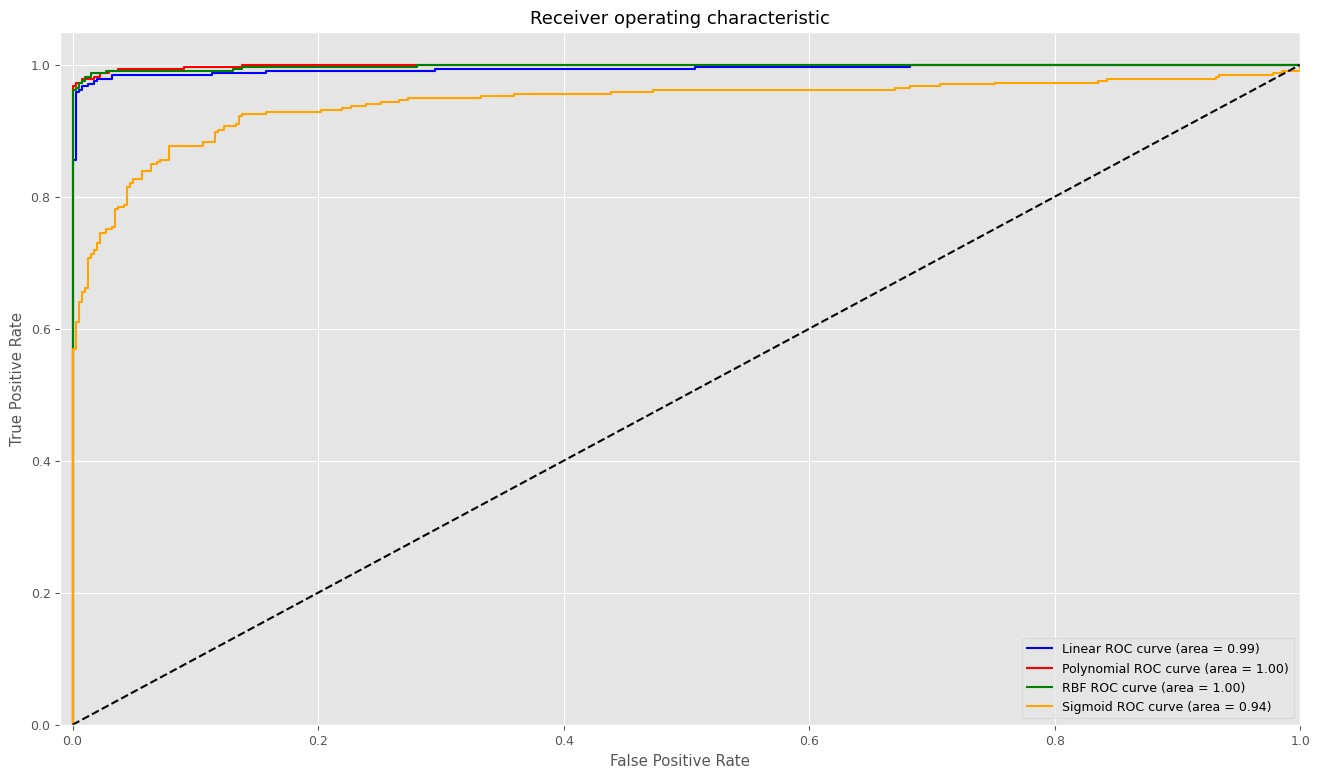
\includegraphics[width=0.75\textwidth]{img/svm/roc_SVM.png}
        \caption{Curva ROC dei vari kernel SVM a confronto}
        \label{fig:roc_SVM_corr}
    \end{figure}

    Dalla tabella \ref{tab:top_metrics_kernels_corr} si può notare che il kernel Rbf
    è quello che ha ottenuto i risultati migliori per tutte le metriche. Inoltre anche
    per il confronto delle curve roc \ref{fig:roc_SVM_corr} Rbf risulta essere il
    migliore anche se i risultati degli altri kernel rimangono ottime opzioni esclusa
    la sigmoide.

\subsection{SVM su dataset con dataset PCA}

% ==============================================================================
\section{Gaussian Naive Bayes}
Di seguito verrà presentato il processo di addestramento del modello
\textbf{Gaussian Naive Bayes}. È importante precisare che la scelta di utilizzare
questo modello è stata fatta con la consapevolezza che non tutte le features
derivano da una distribuzione normale, andando contro le ipotesi del modello.
Tuttavia, abbiamo deciso di utilizzarlo in quanto volevamo distaccarci da un
approccio geometrico e sfruttare un modello probabilistico.
\subsection{Addestramento di Gaussian Naive Bayes}
Come per gli altri approcci, abbiamo deciso di addestrare due modelli, uno su
\texttt{dataset\_corr} e l'altro su \texttt{dataset\_pca}.

La libreria utilizzata per l'implementazione di Gaussian Naive Bayes
presenta come iperparametri solo la definizione delle prior, il problema è che non
essendo esperti del dominio, non possiamo sapere con certezza la probabilità 
di presenza del tumore nei pazienti. Perciò non è stato effettuato un processo di 
ricerca delle prior.

\section{Rete Neurale}
In questa sezione verrà presentata la \textbf{rete neurale}. Nello specifico, si
andranno a presentare i passaggi che sono stati effettuati per la realizzazione
di questo modello, prestando particolare attenzione alla fase di definizione
della struttura della rete neurale e alla fase di addestramento della stessa.

In questo capitolo tutte le operazioni effettuate sono state realizzate
utilizzando i dataset standardizzati (\texttt{dataset\_corr\_std} e
\texttt{dataset\_pca\_std}) presentati nella fase di preparazione dei
dati \ref{sec:riduzione_correlazione}.
\subsection{Struttura della rete neurale}
La fase di definizione della struttura della rete neurale è stata effettuata
attraverso una serie di passaggi. Inizialmente, è stata effettuata un'analisi
dei dati in modo tale da selezionare un sottoinsieme di feature le quali sono
state utilizzate come input della rete neurale. Questo sottoinsieme è stato
selezionato in modo tale da garantire che la rete neurale fosse in grado di
discriminare in modo efficace le due classi.

In seguito, è stata effettuata una fase di grid search per valutare la combinazione
migliore di iperparametri per la rete neurale. Questa fase è stata effettuata
attraverso una cross validation a 5 fold, prendendo in considerazione solamente
i dati del training set.

Dai risultati ottenuti dalla fase di analisi e dal dominio del problema, si è
scelto di utilizzare una rete con una struttura di dimensioni ridotte, in modo
tale da ridurre le possibilità che la rete neurale soffra di overfitting.

Per svolgere il compito di classificazione si è scelto di utilizzare una rete
neurale feedforward, la cui struttura, a meno del layer di input e di output, è
stata definita attraverso il processo di grid search.
\subsubsection{Ottimizzazione degli iperparametri}
Come già accennato in precedenza, la ricerca degli iperparametri della rete neurale
è stata effettuata attraverso un processo di grid search. Questo processo ha
permesso di valutare le prestazioni della rete neurale al variare della funzione
di attivazione, del numero di layer nascosti e del numero di neuroni per ogni
layer nascosto.

Visti i risultati ottenuti nella fase di analisi e la volontà di mantenere i
tempi di addestramento bassi, si è scelto di mantenere una struttura di dimensioni
ridotte per la rete neurale. Per questo motivo, l'operazione di grid search è
stata effettuata prendendo in considerazione un numero di neuroni per layer
tra 5, 10 mentre il numero di layer nascosti è stato valutato tra 1 e 2.

Per quanto riguarda la funzione di attivazione, sono state valutate le seguenti
funzioni di attivazione:
\begin{itemize}
    \item \textit{ReLU}
    \item \textit{Leaky ReLU}
    \item \textit{sigmoid}
\end{itemize}

\begin{figure}[!ht]
    \centering
    \begin{subfigure}[b]{0.3\textwidth}
        \centering
        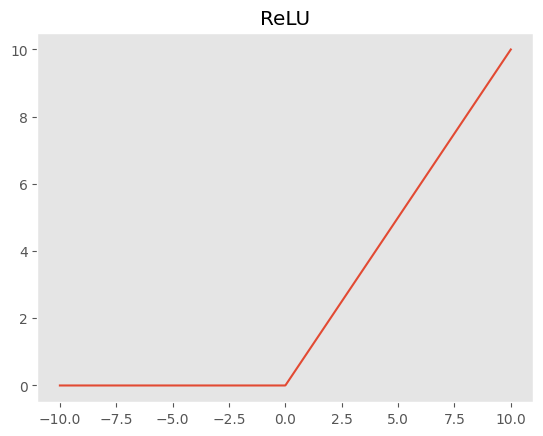
\includegraphics[width=\textwidth]{img/rete/relu.png}
        \caption{ReLU}
        \label{fig:relu}
    \end{subfigure}
    \hfill
    \begin{subfigure}[b]{0.3\textwidth}
        \centering
        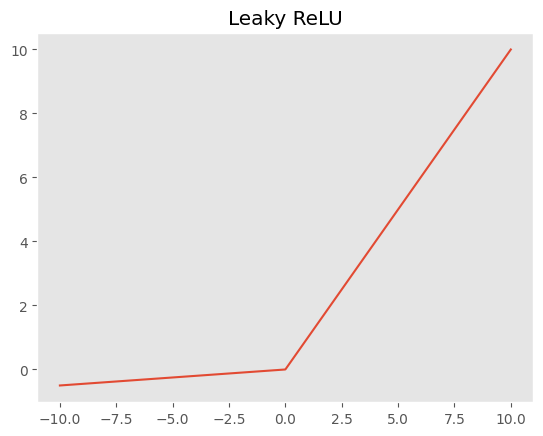
\includegraphics[width=\textwidth]{img/rete/leaky_relu.png}
        \caption{Leaky ReLU}
        \label{fig:leaky-relu}
    \end{subfigure}
    \hfill
    \begin{subfigure}[b]{0.3\textwidth}
        \centering
        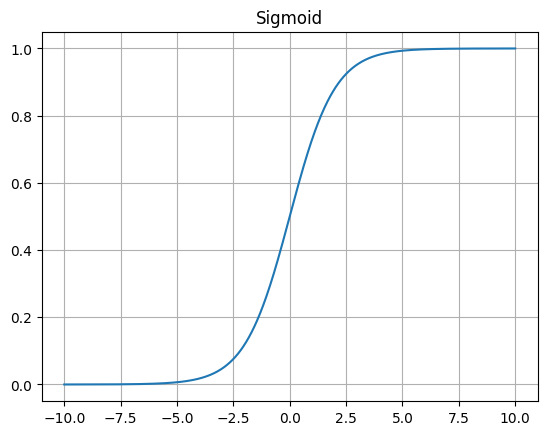
\includegraphics[width=\textwidth]{img/rete/sigmoid.png}
        \caption{Sigmoide}
        \label{fig:sigmoid}
    \end{subfigure}
    \caption{Funzioni di attivazione utilizzate nella fase di grid search}
    \label{fig:}
\end{figure}

Durante il processo di grid search, per ogni modello che è stato addestrato, sono
state raccolte delle informazioni relative all'accuratezza, al tempo di addestramento
richiesto. In aggiunta a queste informazioni, dato che ogni modello è stato
addestrato attraverso una cross validation a 5 fold, sono stati calcolati gli
intervalli di confidenza al $90\%$ per ogni modello addestrato.

Ottenuti i risultati, si è proceduto con l'analisi di questi, in modo tale da
definire la struttura della rete neurale. Per effettuare questa valutazione sono
state utilizzate le misure precedentemente citate.

Il modello selezionato è stato scelto attraverso i seguenti passaggi:
\begin{itemize}
    \item Calcolo della dimensione degli intervalli di confidenza, in modo tale
          da valutare la variabilità delle prestazioni della rete neurale.
          Questa operazione è stata effettuata sia per l'accuratezza che per il
          tempo di addestramento calcolando la differenza tra il massimo e il
          minimo valore dell'intervallo di confidenza.
    \item Assegnazione di un ordinamento per ogni metrica calcolata, in modo tale
          da valutare la posizione di ogni modello nella classifica.
    \item Calcolo del modello migliore attraverso la seguente formula considerando
          la posizione nella classifica di ogni modello per ogni metrica calcolata:
          \begin{center}
              \textit{Modello = 2 * Accuracy + 2 * Tempo di addestramento + 1 * dimensione intervallo di confidenza della Accuracy + 1 * dimensione intervallo di confidenza del Tempo di addestramento}
          \end{center}
\end{itemize}
Le misure di accuratezza e tempo di addestramento si riferiscono alla media
calcolata attraverso la cross validation.

Nello specifico, sono stati utilizzati i seguenti pesi: 2 per l'accuratezza
media, 2 per il tempo di addestramento medio e 1 per gli intervalli di
confidenza. Questi pesi sono stati scelti in modo tale da dare più importanza
all'accuratezza media e al tempo di addestramento medio, in quanto sono le due
misure che permettono di valutare le prestazioni della rete neurale, mentre gli
intervalli di confidenza sono stati utilizzati per valutare la variabilità delle
prestazioni.

Per verificare la validità del modello scelto si è proceduto con il confronto di
esso con la rete che ha ottenuto la migliore accuratezza e quella che ha ottenuto
il tempo di addestramento minore, ottenendo i risultati riportati in tabella \ref{tab:ris-grid-search}.
\begin{table}[ht]
    \centering
    \begin{tabular}{@{}lcc@{}}
        \toprule
        \rowcolor[HTML]{EFEFEF}
        \multicolumn{1}{c}{\cellcolor[HTML]{EFEFEF}\textbf{Modello}} & \textbf{Accuratezza} & \textbf{Tempo di addestramento} \\ \midrule
        Tempo di addestramento minore                                & 97.9\%               & 1.05s                           \\
        Accuratezza maggiore                                         & 99.0\%               & 14.43s                          \\
        Modello scelto                                               & 98.6\%               & 2.59s                           \\ \bottomrule
    \end{tabular}
    \caption{Risultati ottenuti dalla fase di grid search}
    \label{tab:ris-grid-search}
\end{table}

Dai valori riportati nella tabella \ref{tab:ris-grid-search} si può notare che il
notare che il modello che è stato selezionato fornisce un compromesso tra
accuratezza e tempo di addestramento. Nello specifico, perdendo lo $0.4\%$ di
accuratezza si è ottenuto un tempo di addestramento minore di circa $12$ secondi.
\subsubsection{Definizione della struttura della rete neurale}
Dalla fase di analisi è stato selezionato un sottoinsieme di feature le quali
sono state utilizzate come input della rete neurale. Questo sottoinsieme è
composto da 5 elementi, il che ha permesso di definire la struttura del layer di
input della rete neurale, questo primo strato è composto da 5 neuroni, uno per
ogni feature selezionata.

I risultati ottenuti dalla fase di grid search hanno permesso di definire la
struttura della rete neurale. In particolare, la rete neurale è composta da 1
layer di input, 2 layer nascosti e 1 layer di output.

I layer nascosti sono composti nel seguente modo:
\begin{itemize}
    \item Il primo layer nascosto è composto da 10 neuroni, in cui la funzione di
          attivazione è la funzione ReLU \ref{fig:relu}.
    \item Il secondo layer nascosto è composto da 5 neuroni, in cui la funzione
          di attivazione è la funzione ReLU \ref{fig:relu}.
\end{itemize}

Per concludere la descrizione della struttura della rete neurale, è necessario
specificare come è composto l'ultimo layer, ovvero quello di output. Vista la
natura del problema di classificazione, il layer di output è composto da un solo
neurone, in cui la funzione di attivazione è la funzione sigmoide \ref{fig:sigmoid}.
\begin{equation}
    \sigma(x) = \frac{1}{1 + e^{-x}}
\end{equation}
Questa scelta è dovuta al fatto che tale funzione restituisce un valore compreso
tra 0 e 1, il che permette di interpretare l'output della rete neurale come la
probabilità che l'input appartenga alla classe positiva.

La struttura della rete neurale è riassunta nella figura \ref{fig:strutturaReteNeurale}.
\begin{figure}[!ht]
    \centering
    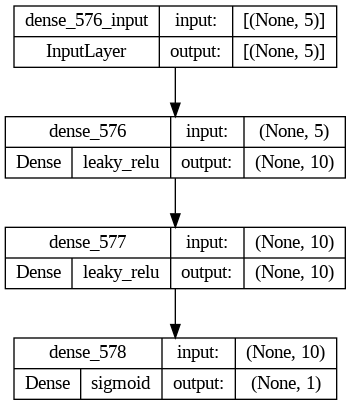
\includegraphics[width=0.3\textwidth]{img/rete/struttura_rete.png}
    \caption{Struttura della rete neurale}
    \label{fig:strutturaReteNeurale}
\end{figure}
\subsubsection{Altri iperparametri}
Oltre alla ricerca della struttura della rete neurale, la fase di grid search è
stata utilizzata per valutare l'algoritmo di ottimizzazione, il numero di epoche
e la dimensione del batch.

Per quanto riguarda l'algoritmo di ottimizzazione, il confronto è stato eseguito
tra \textit{Adam} e \textit{SGD}, mentre per il numero di epoche e la dimensione
del batch sono stati valutati i valori 100, 300 per il numero di epoche e 50,
100, 300 per la dimensione del batch.

I risultati ottenuti dalla fase di grid search hanno permesso di definire i valori
degli iperparametri che hanno permesso di ottenere i migliori risultati. In
particolare, l'algoritmo di ottimizzazione scelto è \textit{Adam}, mentre il
numero di epoche e la dimensione del batch sono stati impostati a 100 e 100
rispettivamente.

In questa fase è stato necessario definire la funzione di perdita. Si è scelta
la \textit{binary crossentropy} in quanto adatta a problemi di classificazione
binaria. La scelta di questa loss è dovuta alla natura del problema di
classificazione che si vuole risolvere.
\subsection{Addestramento della rete neurale}
La fase di addestramento della rete neurale è stata effettuata utilizzando il
training set precedentemente definito. L'addestramento della rete neurale è stato
effettuato utilizzando la libreria \textit{Keras} in quanto permette di definire
e addestrare reti neurali in modo intuitivo.
\subsection{Rete neurale su dataset con PCA}
Per verificare se i risultati ottenuti dal modello addestrato sulle feature da
noi selezionate siano effettivamente dovuti alla struttura delle feature e non
a una fortunata selezione, si è deciso di addestrare un modello con le feature
ottenute attraverso la PCA.

Il dataset ottenuto attraverso la PCA, descritto sella sezione \ref{sec:pca}, è
stato diviso in training set e test set in modo tale da mantenere la stessa
percentuale di dati positivi e negativi in entrambi i set. Oltre a questa
operazione, i dati sono stati standardizzati.
Come per il modello addestrato con le feature selezionate manualmente, anche per
questo modello è stata effettuata una fase di grid search per valutare la
combinazione migliore di iperparametri per la rete neurale.

Il processo utilizzato in questa fase è analogo a quello utilizzato per il modello
precedente, sia a livello di iperparametri che di valutazione del modello.

Come fatto in precedenza, il modello selezionato è stato confrontato con il modello
che ha ottenuto la migliore accuratezza e quello che ha ottenuto il tempo di
addestramento minore. I risultati ottenuti sono riportati in tabella \ref{tab:ris-grid-search-pca}.

\begin{table}[ht]
    \centering
    \begin{tabular}{@{}lcc@{}}
        \toprule
        \rowcolor[HTML]{EFEFEF}
        \textbf{Modello}              & \textbf{Accuratezza} & \textbf{Tempo di addestramento} \\ \midrule
        Tempo di addestramento minore & 96.9\%               & 1.06s                           \\
        Accuratezza maggiore          & 98.0\%               & 22.20s                          \\
        Modello scelto                & 97.9\%               & 1.16s                           \\ \bottomrule
    \end{tabular}
    \caption{Risultati ottenuti dalla fase di grid search}
    \label{tab:ris-grid-search-pca}
\end{table}
Anche in questo caso, come per il precedente, il modello che è stato selezionato
rappresenta un compromesso tra accuratezza e tempo di addestramento. In particolare,
perdendo lo $0.1\%$ di accuratezza si è ottenuto un tempo di addestramento minore
di circa $21$ secondi.


I risultati ottenuti dalla fase di grid search hanno permesso di definire la
struttura della rete neurale. In particolare, la rete neurale è composta da 1
layer di input, 1 layer nascosto e 1 layer di output.

Il layer di input è composto da 3 neuroni, uno per ogni componente principale
ottenuta attraverso la PCA. Questo primo strato è stato definito in questo modo
in quanto il dataset ottenuto attraverso la PCA è composto da 3 feature.

Il layer nascosto è composto da 10 neuroni, in cui la funzione di attivazione è
la funzione ReLU \ref{fig:relu}.

Il layer di output è lo stesso utilizzato per il modello addestrato con le feature
selezionate manualmente, ovvero è composto da un solo neurone, in cui la funzione
di attivazione è la funzione sigmoide \ref{fig:sigmoid}.
\begin{figure}[!ht]
    \centering
    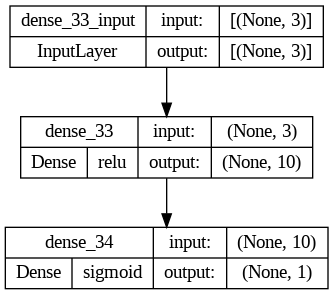
\includegraphics[width=0.3\textwidth]{img/rete/struttura_rete_pca.png}
    \caption{Struttura della rete neurale addestrata con PCA}
    \label{fig:strutturaReteNeuralePCA}
\end{figure}